\section{Experimentación con el filtro neuronal}

A diferencia del filtro adaptativo, el filtro neuronal necesita una etapa de entrenamiento, con lo que la experimentación se llevó a cabo en dos etapas, la primera de entrenamiento y la segunda de evaluación. 

Nuevamente, antes de poder utilizar el filtro neuronal es necesario realizar una calibración de sus parámetros.

\subsection{Parámetros del filtro}

De las ecuaciones vistas en la sección \ref{sec:tecnicas_filtrado_redes_neuronales} se desprende que es necesario definir los siguientes parámetros:

\begin{itemize}
	\item \textbf{L} Tamaño de la ventana en la STFT.
	\item \textbf{N} Tamaño de la DFT usada para computar la STFT o cantidad de muestras en el dominio de la frecuencia en la STFT.
	\item \textbf{R} Solapamiento de ventanas o tasa de muestreo en el tiempo en la STFT.
	\item \textbf{J} Cantidad de ventanas que conforman la STFT o cantidad de muestras en el dominio del tiempo en la STFT. 
	\item Función de error.
	\item Algoritmo de entrenamiento.
	\item Tamaño de los lotes de entrenamiento.
	\item Estructura de la red neuronal.
\end{itemize}

\subsubsection{L Tamaño de la ventana en la STFT}

El tamaño de la ventana en la STFT afecta distintas características del filtrado:

\begin{itemize}
	\item Relación de compromiso entre la resolución en el dominio de la frecuencia y la resolución en el dominio del tiempo. Recordemos de la sección \ref{sec:espectrograma}, que es preferible tener más resolución en tiempo para poder reconocer los distintos sonidos. Por ende mientras más chica sea el tamaño de la ventana mejor.
	\item La señal de audio filtrada se obtiene de a una ventana a la vez, por lo tanto también es preferible una ventana corta para así tener el menor retraso posible.
	\item A medida que la ventana se hace mas chica, a un mismo poder de cómputo, aumenta el tiempo de procesamiento, ya que se necesitan más pasadas por la red neuronal.
\end{itemize}

Como se observa en la descripción anterior, no hay una forma analítica o directa de establecer el tamaño de la ventana. Un valor que se encontró experimentalmente y que mantiene una relación de compromiso adecuada entre los efectos antes mencionados, es de $\SI{16}{ms}$ o $\SI{32}{ms}$. En el presente trabajo se escogió $\SI{16}{ms}$.

Dado que las señales se encuentran muestreadas a $16 Khz$, esto nos da un largo de ventana igual a:

\begin{equation*}
	L = \SI{16}{ms} \cdot \SI{16}{KHz} = 256
\end{equation*}

\subsubsection{N Cantidad de muestras en el dominio de la frecuencia en la STFT}
\label{sec:cantidad_muestras_frecuencia}

La tasa de muestreo en frecuencia afecta las siguientes características:

\begin{itemize}
	\item A medida que aumentamos la tasa de muestreo en frecuencia, mayor resolución tendremos en ella.
	\item A medida que aumentamos la resolución en frecuencia aumenta el tiempo de cómputo de la FFT y aumenta la cantidad de parámetros de las capas convolucionales de la red neuronal.
	\item Recordemos de la sección \ref{sec:muestreo_en_tiempo_y_frecuencia} que $R \leq L \leq N$, es decir $N \ge 256$.
\end{itemize}

Nuevamente tenemos una relación de compromiso que debemos mantener en el nivel adecuado. Para el presente trabajo se utilizó una FFT de $2^{10} = 1024$ puntos. 

\subsubsection{R Solapamiento de ventanas en la STFT}

En la sección \ref{sec:overlapp_and_and} vimos que una elección que permite recuperar la señal de entrada dada la STFT, es utilizar una ventana de Hamming que cumpla la relación $R = L/2$. Dado que en nuestro caso tenemos $L = 256$, obtenemos que $R=128$. Con este valor de $R$ también verificamos la condición necesaria $R \leq L \leq N$, ya que tenemos $128 \leq 256 \leq 1024$.

\subsubsection{J Cantidad de muestras en el dominio del tiempo en la STFT}
\label{sec:ventanas_en_espectrogramas}

La cantidad de ventanas a incluir en cada espectrograma, define qué tanta información hacia atrás en el tiempo puede ver la red neuronal, para predecir la ventana de señal de habla filtrada en el tiempo i. 

Al aumentar o disminuir la cantidad de ventanas $J$ tendremos que:

\begin{itemize}
	\item A mayor cantidad de ventanas, más información tendrá la red para predecir y por ende menor el error de predicción. También, más grande es la dimensión del espectrograma y por ende mayor será la cantidad de parámetros de las capas convolucionales de la red neuronal.
	\item A partir de cierto punto difuso no tiene sentido seguir aumentando la cantidad de ventanas, ya que la ventana en el tiempo $i$ deja de estar correlacionada con la ventana $i - J - 1$ y por ende, no hay información útil que la red pueda utilizar en la predicción de la ventana $i$.
\end{itemize}

Experimentalmente se encontró que un número razonable de ventanas es $J=64$.

\subsubsection{Función de error o función de costo}

La función de error define la medida que se busca minimizar durante el entrenamiento de la red. El objetivo de esta función es, permitir ajustar los pesos de la red de tal manera que la medida sea cada vez más chica. En nuestro caso, a la salida de la red tenemos una ventana de la señal filtrada en el dominio de la frecuencia y como valor objetivo tenemos una ventana de la señal de habla sin ruido, también en el dominio de la frecuencia. La función de costo calcula el error entre lo obtenido a la salida de la red y el valor objetivo. 

La función de costo más adecuada para la tarea en cuestión es el error cuadrático medio:

\begin{equation*}
	l = \frac{1}{K} \sum_{i=1}^K (Y(n_i, w_i) - X(n_i, w_i))^2
\end{equation*}

\subsubsection{Algoritmo de entrenamiento}

Para poder entrenar la red neuronal es necesario escoger un optimizador. Los optimizadores se pueden ver como funciones que definen la metodología en la que se van a actualizar los pesos de la red. En el caso de los filtros adaptativos, los distintos tipos de optimizadores utilizados dan lugar a distintos filtros como el LMS, el NLMS, el RLS, etc.

Dos algoritmos, comúnmente utilizados para entrenar redes neuronales, son el método de gradiente estocástico con momento \cite{deep_learning} y el método Adam \cite{adam_optimizer}. Usualmente, el método Adam converge mas rápido gracias al uso de momentos de segundo orden.

Configurar correctamente los hiper-parámetros del optimizador resulta esencial para poder minimizar, tanto el error durante el entrenamiento como el error de generalización.

Para escoger el optimizador adecuado se evaluaron ambos experimentalmente y con Adam se obtuvieron mejores resultados, con respecto al error de generalización y la velocidad de entrenamiento. 

El optimizador Adam depende de tres hiper-parámetros, $\eta$, $\beta_1$ y $\beta_2$. El parámetro $\eta$ define la tasa de aprendizaje y los parámetros $\beta_1$ y $\beta_2$ permiten ajustar las estimaciones del valor medio y la varianza del gradiente de la función de error. Para el presente trabajo los valores utilizados fueron: $lr=1e^{-4}$, $\beta_1=0.9$ y $\beta_2=0.999$.

\subsubsection{Tamaño de los lotes de entrenamiento}

El tamaño de lote de entrenamiento define cuántas muestras deben pasar por la red, antes de calcular el error y ajustar los pesos o parámetros. El rango en el que debe estar el tamaño de lote es entre una muestra y el tamaño del conjunto de entrenamiento completo. En general, en lo referido al entrenamiento de redes neuronales, se suele utilizar el concepto de \emph{mini-batch}, es decir un lote pequeño. 

Idealmente, el tamaño del lote debería ser el conjunto de entrenamiento completo pero esto trae varios problemas.

\begin{itemize}
	\item Se ha demostrado experimentalmente que tamaños de lotes grandes afectan negativamente el error de generalización de la red \cite{on_large_batch_training}.
	\item Un lote grande requiere mucha memoria, la cual suele ser limitada en especial cuando el entrenamiento se lo realiza en una o mas GPUs.
\end{itemize}

Por otro lado, si el tamaño de lote es muy pequeño, el algoritmo de optimización no logra encontrar la dirección de minimización. En estos casos, el gradiente presenta una gran variación muestra a muestra.

Por último, en nuestro caso, debemos también tener en cuenta que una señal de habla no es la muestra que ingresa a la red sino que lo que ingresa a la red son espectrogramas de esa señal de habla. Las señales de habla utilizadas en el presente trabajo tienen en promedio 80 espectrogramas. Es esencial para el entrenamiento adecuado de la red, que antes de cada actualización de los parámetros se haya pasado por la red muestras de distintos audios, de lo contrario el optimizador no logrará encontrar la dirección de minimización. En el presente trabajo, durante el entrenamiento, se utilizó un tamaño de lote de $256$ muestras.

\subsubsection{Estructura de la red neuronal}

En la sección \ref{sec:cantidad_muestras_frecuencia} vimos que el largo de la DFT utilizada para el cómputo de la STFT es de $N=1024$. Las señales de habla son señales reales, con lo cual la DFT tendrá simetría conjugada, esto nos lleva a que la información espectral esté duplicada.

Utilizar toda la DFT es innecesario e implicaría un tiempo de cómputo mayor. Debido a la simetría que presenta, toda la información útil de la DFT la podemos encontrar en cada una de las mitades de la simetría. Esto nos lleva a que los espectrogramas que sirven como entrada a la red están conformados por $512$ muestras en el dominio de la frecuencia.

Por otro lado, en la sección \ref{sec:ventanas_en_espectrogramas}, vimos que la cantidad de ventanas a incluir en un espectrograma es de $J=64$. Esto nos lleva a obtener el tamaño de los espectrogramas, el cual es de $512 \times 64$. El tamaño de los espectrogramas resulta esencial para definir la estructura de la red.

Como vimos en la sección \ref{sec:redes_tipo_u}, a medida que los espectrogramas pasan por las distintas capas de la red, el tamaño se irá reduciendo hasta terminar el camino del codificador. Luego, pasan a la parte del decodificador, donde el tamaño se va recuperando capa a capa. En el codificador, a medida que se reduce el tamaño se aumenta la cantidad de filtros presentes en la capa convolucional. En el decodificador, a medida que se aumenta el tamaño, se reduce la cantidad de filtros.

En la figura \ref{fig:ch7_red_estructura} podemos ver cómo se va modificando el tamaño de los espectrogramas a medida que pasan por las distintas capas de la red. La notación es \textbf{Tamaño en frecuencia} $\times$ \textbf{Tamaño en tiempo} $\times$ \textbf{Canales}. Cada canal representa el resultado de la convolución entre la entrada y uno de los filtros de la capa.

\begin{figure}
	\centering
	\centerline{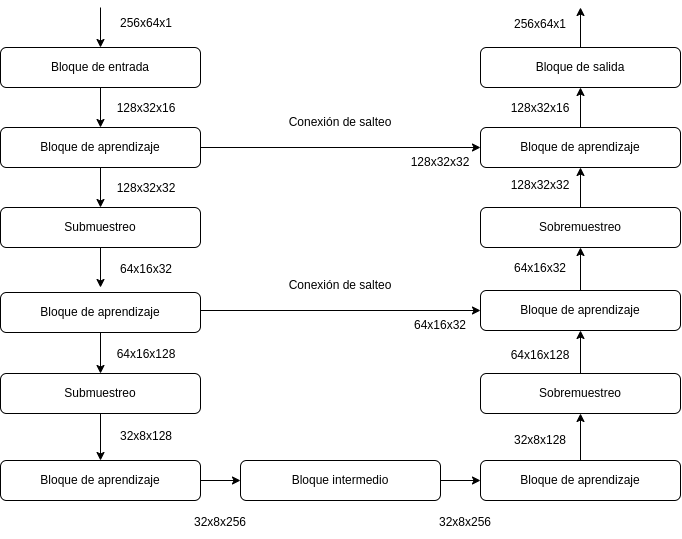
\includegraphics[scale=0.65]{images/ch7/red_estructura.png}}
	\caption{Estructura del filtro neuronal.}
	\label{fig:ch7_red_estructura}
\end{figure}

\subsection{Entrenamiento}

El entrenamiento de la red consiste en pasar por ella espectrogramas de señales ruidosas, obtener el error respecto de los espectrogramas de las señales sin ruido y modificar los pesos de la red de acuerdo a ese error.

Usualmente, durante el entrenamiento, se le muestra a la red más de una vez cada muestra del conjunto de entrenamiento. Es posible que después de cierto punto, la red empiece a aprenderse por fuerza bruta el conjunto de entrenamiento con lo que el error de generalización comienza a aumentar. Para poder detectar este momento se suele introducir una etapa de validación cada x lotes de entrenamiento. La validación se hace contra el conjunto de validación, el cual es un subconjunto del conjunto de pruebas.

Durante el entrenamiento se evaluó el desempeño de tres métricas:

\begin{enumerate}
	\item El error cuadrático medio entre la salida de la red y el espectrograma sin ruido alineado con la entrada.
	\item El error porcentual absoluto medio MAPE (por sus siglas en inglés) nuevamente entre la salida de la red y el espectrograma sin ruido alineado con la entrada. \label{item:mape}.
	\item El MAPE entre las señales de audio construidas a partir de las salidas de la red y la señal de habla original. \label{item:audio_mape}
\end{enumerate}

El MAPE se obtiene como:

\begin{equation*}
	\frac{1}{n} \sum_{\forall i} \left| \frac{y_i - s_i}{y_i} \right|
\end{equation*}

donde $y$ es el valor obtenido y $s$ la señal esperada.

Para las métricas \ref{item:mape} y \ref{item:audio_mape}, además, se computó un límite superior dado por la señal de habla sin ruido y la señal de habla ruidosa.

En las figuras \ref{fig:ch7_entrenamiento_mse} y \ref{fig:ch7_validacion_mse} podemos ver el error cuadrático medio durante el entrenamiento y durante la validación.

\begin{figure}
	\centering
	\centerline{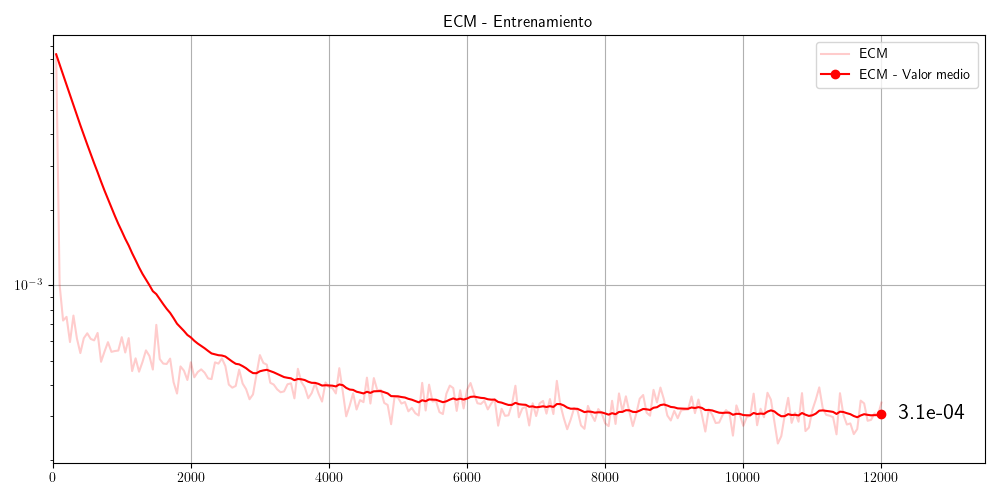
\includegraphics[scale=0.65]{images/ch7/entrenamiento/train_mse.png}}
	\caption{Error cuadrático medio durante el entrenamiento.}
	\label{fig:ch7_entrenamiento_mse}
\end{figure}

\begin{figure}
	\centering
	\centerline{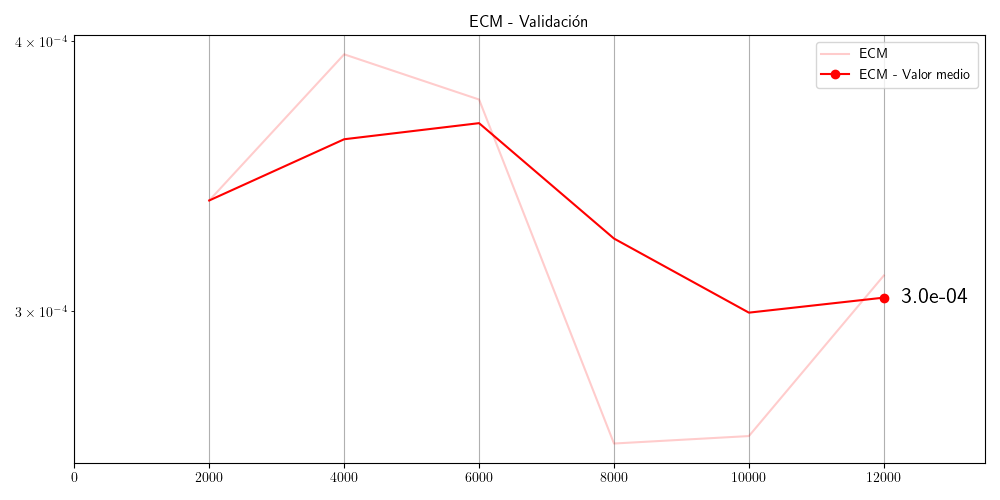
\includegraphics[scale=0.65]{images/ch7/entrenamiento/val_mse.png}}
	\caption{Error cuadrático medio durante la validación.}
	\label{fig:ch7_validacion_mse}
\end{figure}

La validación se ejecutó cada 2.000 lotes de entrenamiento y se realizó sobre un total de 500 audios.

Como se puede ver en la figura \ref{fig:ch7_validacion_mse}, en trazo claro, el error de generalización comenzó a aumentar en el número de lote 8.000 y el aumento fue confirmado en los lotes 10.000 y 12.000, por lo que el entrenamiento fue frenado. Dado que a partir del lote 8000, el error comenzó a aumentar, el modelo seleccionado fue el obtenido en el lote 8.000 y se descartaron los modelos de los lotes 10.000 y 12.000.

Por otro lado, es imprescindible contar con métricas como la \ref{item:mape} y \ref{item:audio_mape} para poder observar si el modelo de red obtenido en cada iteración, logra mejorar los errores de referencia obtenida por medio de la señal de habla original y la señal de habla ruidosa ruidosa. En las figuras \ref{fig:ch7_entrenamiento_mape}, \ref{fig:ch7_val_mape}, \ref{fig:ch7_entrenamiento_audio_mape} y \ref{fig:ch7_val_audio_mape} podemos encontrar el resultado de tales métricas.

\begin{figure}
	\centering
	\centerline{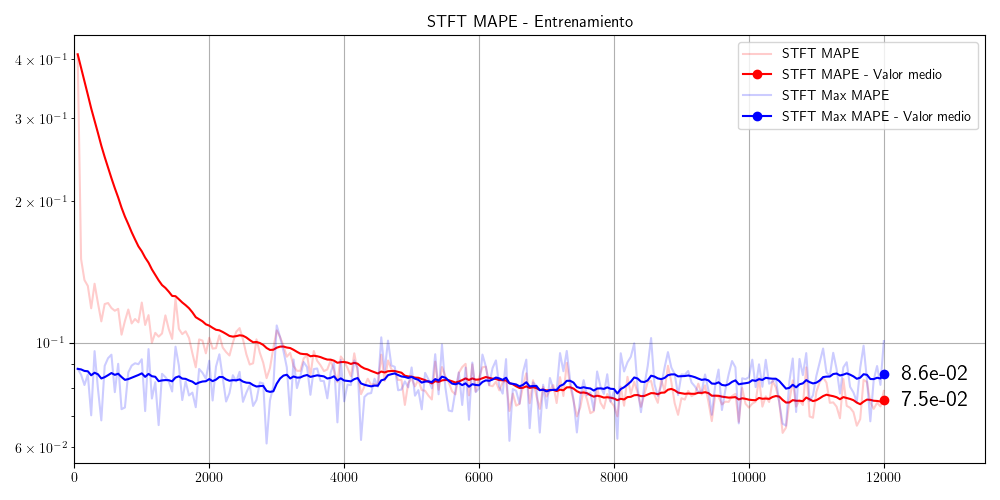
\includegraphics[scale=0.65]{images/ch7/entrenamiento/train_stft_mape.png}}
	\caption{MAPE durante el entrenamiento.}
	\label{fig:ch7_entrenamiento_mape}
\end{figure}

\begin{figure}
	\centering
	\centerline{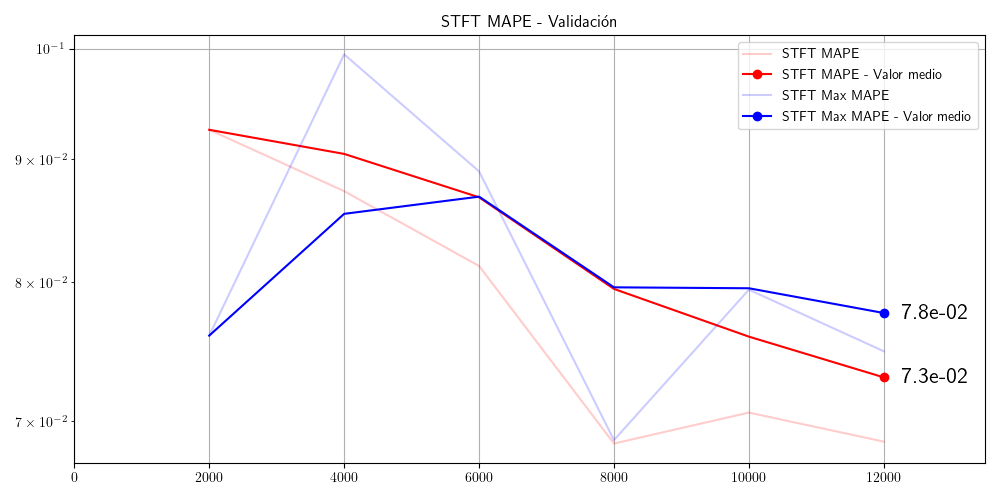
\includegraphics[scale=0.65]{images/ch7/entrenamiento/val_stft_mape.png}}
	\caption{MAPE durante la validación.}
	\label{fig:ch7_val_mape}
\end{figure}

\begin{figure}
	\centering
	\centerline{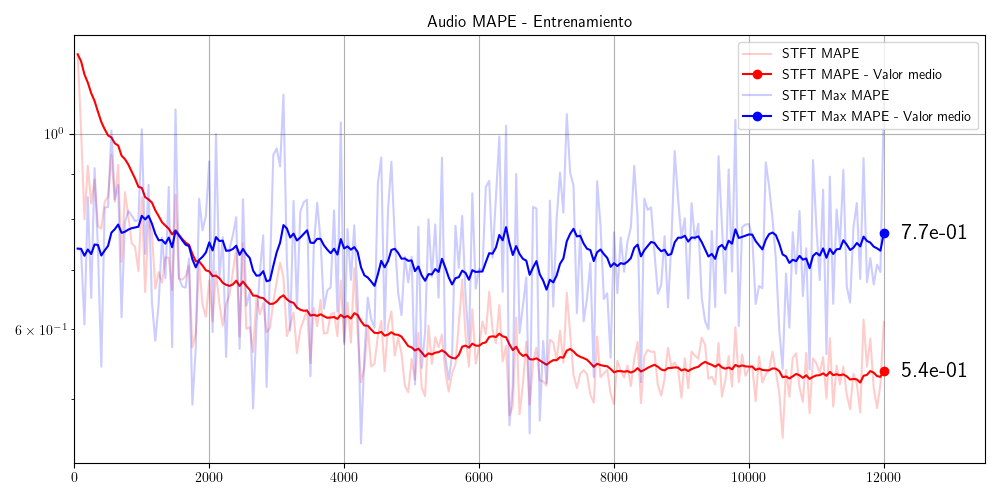
\includegraphics[scale=0.65]{images/ch7/entrenamiento/train_audio_mape.png}}
	\caption{MAPE en las señales de audio durante el entrenamiento.}
	\label{fig:ch7_entrenamiento_audio_mape}
\end{figure}

\begin{figure}
	\centering
	\centerline{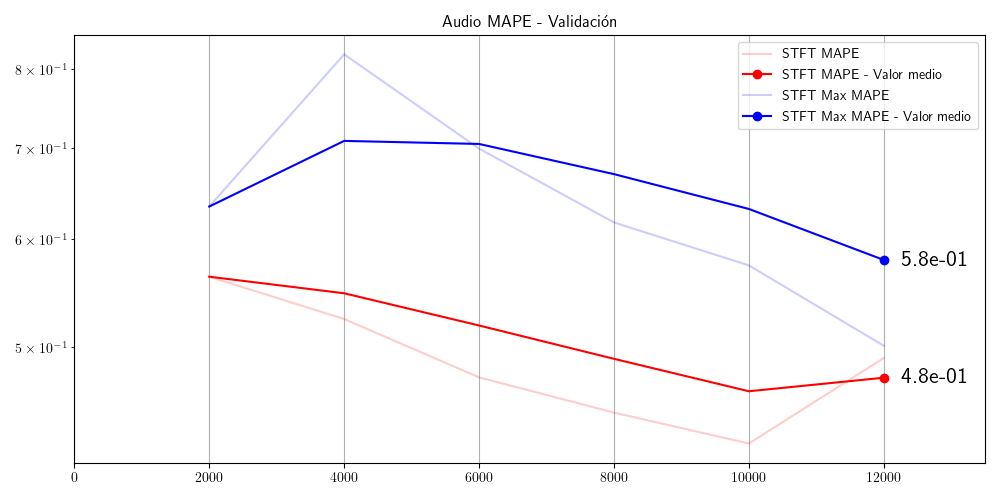
\includegraphics[scale=0.65]{images/ch7/entrenamiento/val_audio_mape.png}}
	\caption{MAPE en las señales de audio durante la validación.}
	\label{fig:ch7_val_audio_mape}
\end{figure}

En las figuras \ref{fig:ch7_val_mape} y \ref{fig:ch7_val_audio_mape} podemos ver que, aproximadamente después del lote 3.000, los errores en el conjunto de validación ya estaban por debajo de su cota máxima, con lo cual podemos estar seguros que el modelo de red obtenido en el lote 8000 ya va a haber logrado filtrar parcial o totalmente el ruido presente en las señales de habla ruidosas.

\subsection{Resultados}
\label{sec:resultados_filtro_neuronal}

\subsubsection{Medida PESQ}

Al igual que para el caso del filtro adaptativo, se puso a prueba el desempeño del filtro neuronal en el conjunto de pruebas, computando las mismas medidas PESQ para cada uno de los niveles de ruido utilizados. 

En la figura \ref{fig:ch7_pesq_resume} podemos ver la medida $\Delta \textbf{PESQ Valor medio}$ en función del nivel de ruido. Se observa que la máxima mejora media en PESQ se logra para los $\SI{15}{dB}$, y tanto para SNRs menores como mayores, la mejora media en la PESQ disminuye, siempre manteniéndose positiva. En la siguiente sección se analiza este comportamiento en detalle.

\begin{figure}
	\centering
	\centerline{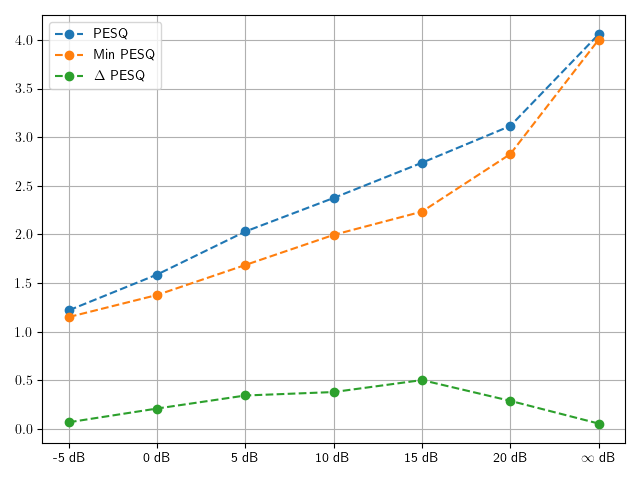
\includegraphics[scale=0.70]{images/ch7/objective_metrics/metric_PESQ.png}}
	\caption{PESQ en función de la SNR.}
	\label{fig:ch7_pesq_resume}
\end{figure}

En el cuadro \ref{table:neural_filter_pesq_resume} podemos ver los mismos resultados que en la figura \ref{fig:ch7_pesq_resume} pero en valores porcentuales:

\begin{table}[ht]
	\centering
	\begin{tabular}{ |c|c|c|c|c|c|c|c| } 
		\hline
		SNR [dB] & $-5$ & $0$ & $5$ & $10$ & $15$ & $20$ & $\inf$ \\ 
		\hline
		$\Delta \textbf{PESQ Valor medio}$ & 6\%  & 15\%  & 20\% & 19\% & 22\% & 10\% & 2\% \\
		\hline
	\end{tabular}
	\caption{Medida $\Delta \textbf{PESQ Valor medio}$ para cada valor de SNR.}
	\label{table:neural_filter_pesq_resume}
\end{table}

En la figura \ref{fig:ch7_pesq_resume_by_noise} podemos ver le medida PESQ en función del tipo de ruido. 

\begin{figure}
	\centering
	\centerline{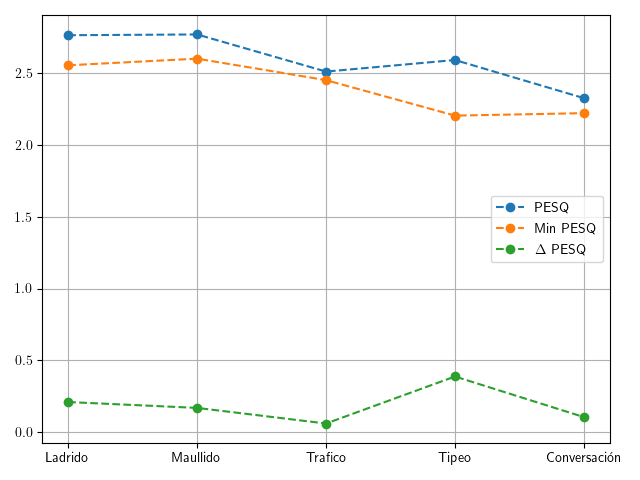
\includegraphics[scale=0.75]{images/ch7/dnn_metric_PESQ_noises.png}}
	\caption{PESQ en función del tipo de ruido.}
	\label{fig:ch7_pesq_resume_by_noise}
\end{figure} 

En el ruido de la clase \emph{Tipeo}, el filtro neuronal logra un buen desempeño y en los tipos \emph{Tráfico} y \emph{Conversación} no logra una mejora sustancial. Estos dos últimos tipos de ruidos son los mas complejos para ser filtrados por la red neuronal, debido a la complejidad del ruido en si mismo. 

En el ruido \emph{Conversación} hay personas hablando, cuyas voces se mezclan con la señal de habla principal, dificultándole a la red identificar cuál es la señal a filtrar.

El ruido \emph{Tráfico} tiene una complejidad inherente, debido a la gran variedad de sonidos que se pueden encontrar en la vía pública. En el otro extremo, el ruido \emph{Tipeo} es relativamente simple y le resulta sencillo a la red neuronal caracterizarlo y filtrarlo.


\subsubsection{Medida STOI}

Se puso a prueba el desempeño del filtro neuronal en el conjunto de pruebas, computando las medidas STOI ya definidas para cada uno de los niveles utilizados. 

En la figura \ref{fig:ch7_stoi_resume} podemos ver la medida $\Delta \textbf{STOI Valor medio}$ en función del nivel de ruido. Se observa que la máxima mejora media en STOI se logra para los $\SI{5}{dB}$, y tanto para SNRs menores como mayores, la mejora media en la STOI disminuye.

\begin{figure}
	\centering
	\centerline{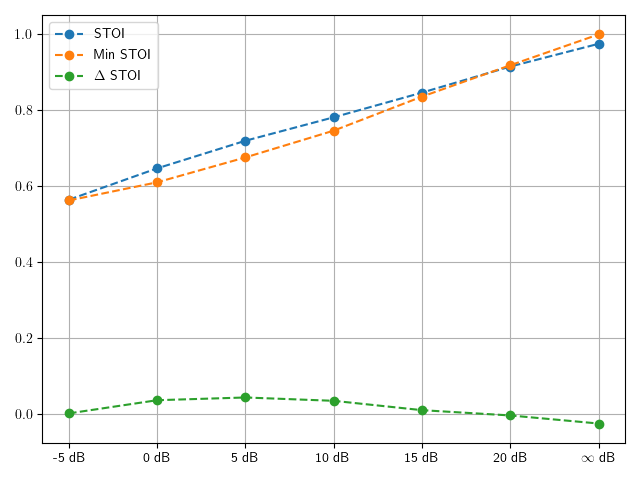
\includegraphics[scale=0.70]{images/ch7/objective_metrics/metric_STOI.png}}
	\caption{STOI en función de la SNR.}
	\label{fig:ch7_stoi_resume}
\end{figure}

En el cuadro \ref{table:neural_filter_stoi_resume} podemos ver los mismos resultados que en la figura \ref{fig:ch7_stoi_resume} pero en valores porcentuales:

\begin{table}[ht]
	\centering
	\begin{tabular}{ |c|c|c|c|c|c|c|c| } 
		\hline
		SNR [dB] & $-5$ & $0$ & $5$ & $10$ & $15$ & $20$ & $\inf$ \\ 
		\hline
		$\Delta \textbf{STOI Valor medio}$ & 0\%  & 6\%  & 6\% & 5\% & 1\% & 0\% & -2\% \\
		\hline
	\end{tabular}
	\caption{Medida $\Delta \textbf{STOI Valor medio}$ para cada valor de SNR.}
	\label{table:neural_filter_stoi_resume}
\end{table}

En la figura \ref{fig:ch7_stoi_resume_by_noise} podemos ver le medida PESQ en función del tipo de ruido. Nuevamente, la red se destacó en el ruido del tipo \emph{Tipeo} pero en las demás clases de ruido no logró una mejora sustancial.

\begin{figure}
	\centering
	\centerline{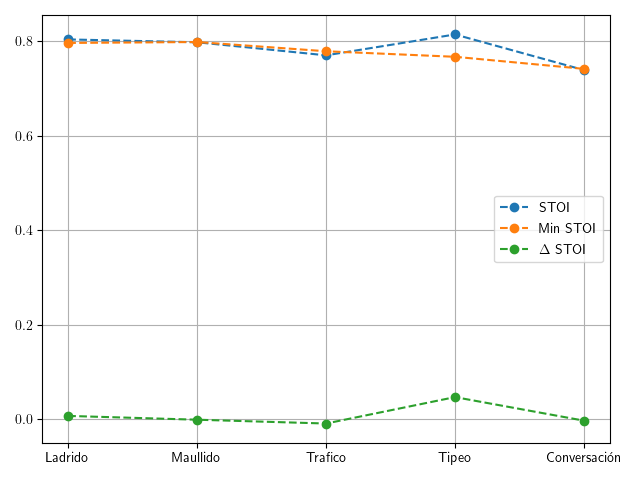
\includegraphics[scale=0.75]{images/ch7/dnn_metric_STOI_noises.png}}
	\caption{STOI en función del tipo de ruido.}
	\label{fig:ch7_stoi_resume_by_noise}
\end{figure} 

\subsubsection{Error cuadrático medio y nivel de ruido}

Dada la señal de habla sin ruido $s_p(n)$, la señal filtrada $\hat{s}_p(n)$ y la cantidad de señales de audio $P$, en la base de datos de pruebas, así como con el filtro adaptativo, se computa el error cuadrático medio:

\begin{equation*}
	\text{ECM}(n) = \frac{1}{P-1} \sum_{p=0}^{P} (\hat{s}_p(n) - s_p(n))^2
\end{equation*}

\noindent y el nivel de ruido medio al cuadrado:

\begin{equation*}
	\text{Nivel de ruido}(n) = \frac{1}{P-1} \sum_{p=0}^{P} (n_p(n))^2
\end{equation*}

A diferencia del filtro adaptativo, donde había una correlación directa entre el ECM y las medidas PESQ y STOI, en el filtro neuronal no sucede lo mismo como se puede observar en la figura \ref{fig:ch7_mse_and_noise_level}. En esta gráfica se muestra el error cuadrático medio y el nivel de ruido, promediado para todo $n$ en función de la SNR. 

Podemos observar, que a bajos niveles de SNR, el ECM no es comparable con el nivel de ruido pero si lo es a altos niveles. Sin embargo, en las figuras \ref{fig:ch7_pesq_resume} y \ref{fig:ch7_stoi_resume} vimos que, tanto en bajos niveles de SNR como en altos, el filtro no logró mejorar sustancialmente las medidas PESQ y STOI.

\begin{figure}
	\centering
	\centerline{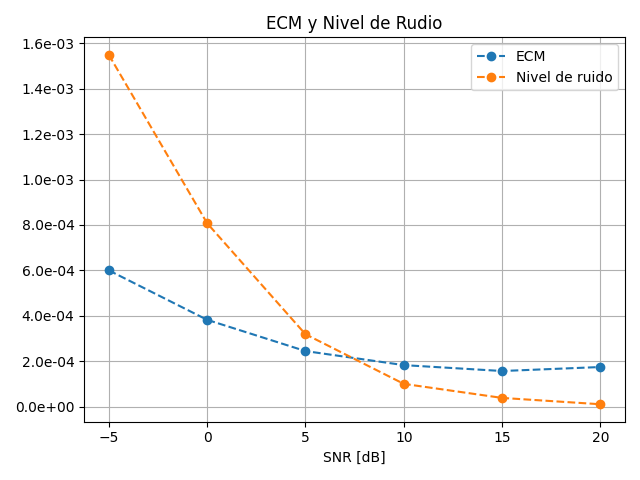
\includegraphics[scale=0.30]{images/ch7/ecm_and_noise_level.png}}
	\caption{ECM y Nivel de ruido.}
	\label{fig:ch7_mse_and_noise_level}
\end{figure}


El filtro neuronal, al trabajar en el dominio de la frecuencia, se ve mayormente afectado en las medidas PESQ y STOI por los errores de estimación que en el caso del filtro adaptativo. En el filtro neuronal, a bajos niveles de SNR, los errores de estimación en el espectro de la señal filtrada  afectan en gran proporción las medidas PESQ y STOI, debido al alto contenido de ruido presente en la señal de entrada.

A altos niveles de SNR, los errores de estimación no afectan en gran proporción las medidas PESQ y STOI debido a que el contenido de ruido es bajo. Sin embargo, como se observa en la figura \ref{fig:ch7_mse_and_noise_level}, a altos niveles de SNR el error de estimación o el error de generalización de la red \cite{deep_learning} se vuelve comparable con nivel de ruido. Esto genera que nuevamente las medidas PESQ y STOI sean cercanas a cero como sucedió en el caso del filtro adaptativo.